\chapter{4TH INDUSTRIAL [R]EVOLUTION}
\label{ch:Fourth}

The fourth industrial revolution builds on the second wave of digitization, representing new ways in which technology becomes embedded within societies and the human mind and body. The Fourth Industrial Revolution is marked by emerging technology breakthroughs in several fields, including blockchain, robotics, artificial intelligence, nanotechnology, quantum computing, biotechnology, The Internet of Things (IoT), 3D printing and autonomous vehicles (\cref{fig:mapping global transformation}).

    \begin{figure}
    \centering
    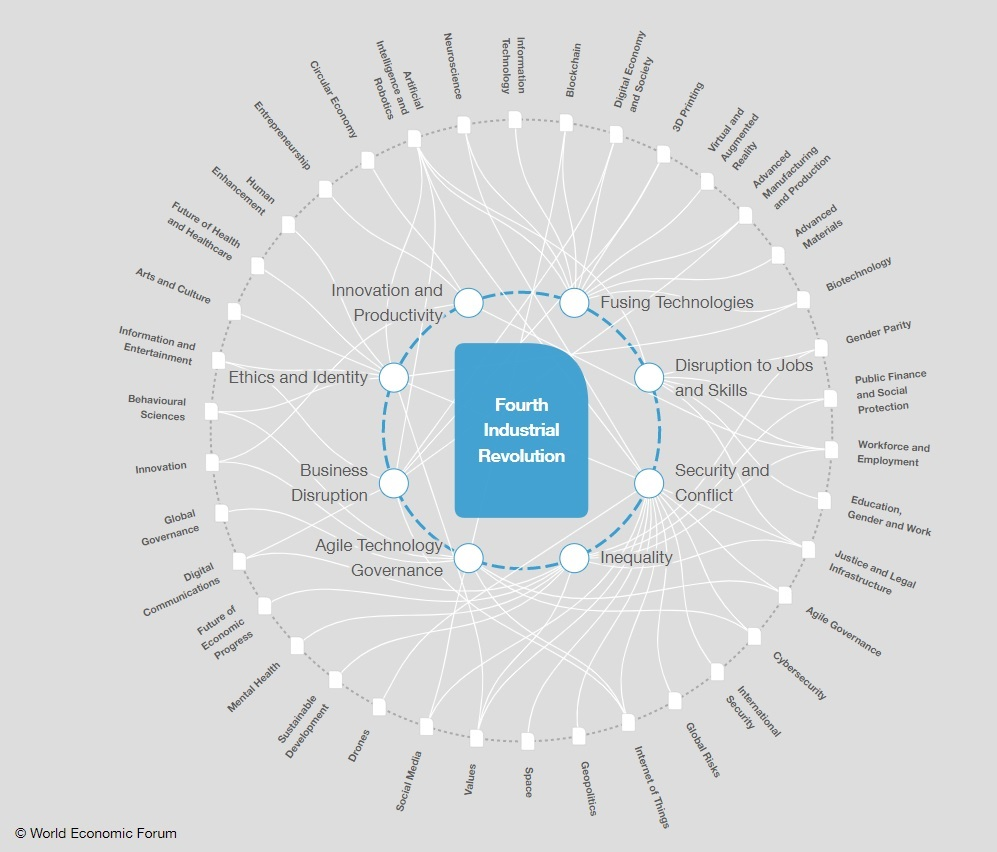
\includegraphics[width=.9\textwidth]{img/ch-revolution/WEF_fourth_industrial_revolution.jpg}
    \caption{Fourth Industrial Revolution. Mapping global transformations tool.}
    \source{World Economic Forum. \emph{Mapping Global Transformations.} \cite{Global_Transformations}}
    \label{fig:mapping global transformation}
    \end{figure}

    
    \section{Exponential science}
    
    There are several significant indicators why this transformation does not merely reflect a continuation of the Third Industrial Revolution but heralds something wholly new and unique. At present we live in a globalized, profoundly connected and intertwined world and it is changing rapidly. The speed, scope and impact of this transformation are unprecedented. The fourth Industrial Revolution is everywhere around us, and it is progressing at an exponential pace.
    
    Throughout our history, breakthrough technological advances were few and far between. It is only until the last decennia that we have reached the unparalleled speeds at which we are currently progressing in every direction.
    
    Rapidly changing technology is not only affecting how we live our lives but also the way we communicate and do business with each other. The coming years will be of crucial importance as governmental bodies, regulators and legislators might not keep up with the rapid changes in technology and infrastructure and seek to contain or prohibit its uses. 
   
    
    \begin{quotation}

      \textit{\say{Technology goes beyond mere tool making; it is a process of creating ever more powerful technology using the tools from the previous round of innovation.}}
      \begin{flushright}
        \small{--- \textbf{Kurzweil, Ray}}
      \end{flushright}
    
    \end{quotation}
    
    Everybody will be aware of the ongoing debate around big-data and data monopolies by large technology companies such as Amazon, Google and Facebook. It is not a surprise that privacy and online security must be considered to be one of the most pressing challenges which we will have to face. Daily, we are donating valuable data to technology giants. While we all seem to understand that this is very alarming, we know it is an essential part of our relatively new and interconnected lifestyle. We seem to be hesitant when it comes to giving up our luxuries of the 20th century. 
    
    However, what we lack is healthy competition to counteract these data monopolies. Smaller companies instantly get bought up and are assimilated when considered a threat to the monopolistic business model. New players - making use of decentralized and open-source technology have now entered the arena and are preparing to take on the fight.
    
    \begin{quotation}

  \textit{\say{Debates about fundamental issues such as the impact on our inner lives of the loss of control over our data will only intensify in the years ahead. Similarly, the revolutions occurring in biotechnology and AI, which are redefining what it means to be human by pushing back the current thresholds of life span, health, cognition, and capabilities, will compel us to redefine our moral and ethical boundaries.}}
  \begin{flushright}
    \small{--- \textbf{Schwab, Klaus}}
  \end{flushright}

\end{quotation}
    

    \section{Fusing technologies}
    
    The Fourth Industrial Revolution has very distinctive features when compared with the industrial revolutions we have witnessed in the past. A crucial characterization is that it builds upon the fusion of (new) technologies, and there is increasing compatibility between - and collaboration of - various research disciplines.
    
    The main catalysts of this phenomenon are our ever-increasing digital capabilities.
    Almost every new scientific development or breakthrough now uses and leverages digital capability. It is tough to come up with examples of non-digital technology in our digital world. Computers, processing chips and algorithms are everywhere.\medskip
    
    For example, advances in biotechnology such as genome editing and potential brain-machine interfaces, would not have been possible without significant increases in computing power and increased data gathering and data analysis. Following the same trend, sophisticated robotics and artificial intelligence (AI) would not exist if not thanks to massive improvements and innovations in the field of computing and processing power and further digitization. Apart from our mobile phones, personal computers and laptops, our physical world has numerous interfaces with the digital world. Think about autonomous vehicles (cars, drones and ships), smart-homes and industrial-scale manufacturing processes utilizing 3D printing.\medskip
  

    \section{Internet of Things}
    Furthermore, the rise of the Internet of Things (IoT) and the corresponding advances in sensing (sensor) technology is enabling our autonomous systems to improve their understanding of the environment in real-time. Ultimately robots will no longer only exist on factory floors where they mindlessly operate the assembly lines. Robots and artificial intelligence will evolve, and new technology will empower them to perform more diverse and broad ranges of tasks.    
  
    These systems are now able to access real-time information remotely via the cloud and connect to exchange and analyze data and learn collectively (\cref{fig:IOTsensors.jpg}). In the age of the Internet of Things (IoT), there will be an increasing emphasis on real-time data gathering, data analyses and human-machine collaboration.
    \medskip
    
  \tcbset{colback=orange!3!white,fonttitle=\bfseries}
    \begin{tcolorbox}
    [enhanced,
    title=Global nervous system,
    frame style=
    {left color=orange!85!black,right color=yellow!95!black}]
        
                \textit{\say{The internet gave us the possibilities to connect in ways we would never have dreamed possible. The Internet of Things will take us beyond the connection to become part of a living, breathing and moving global nervous system.}}
               
\end{tcolorbox}
\medskip

    
    
    \begin{figure}[hb]
    \centering
    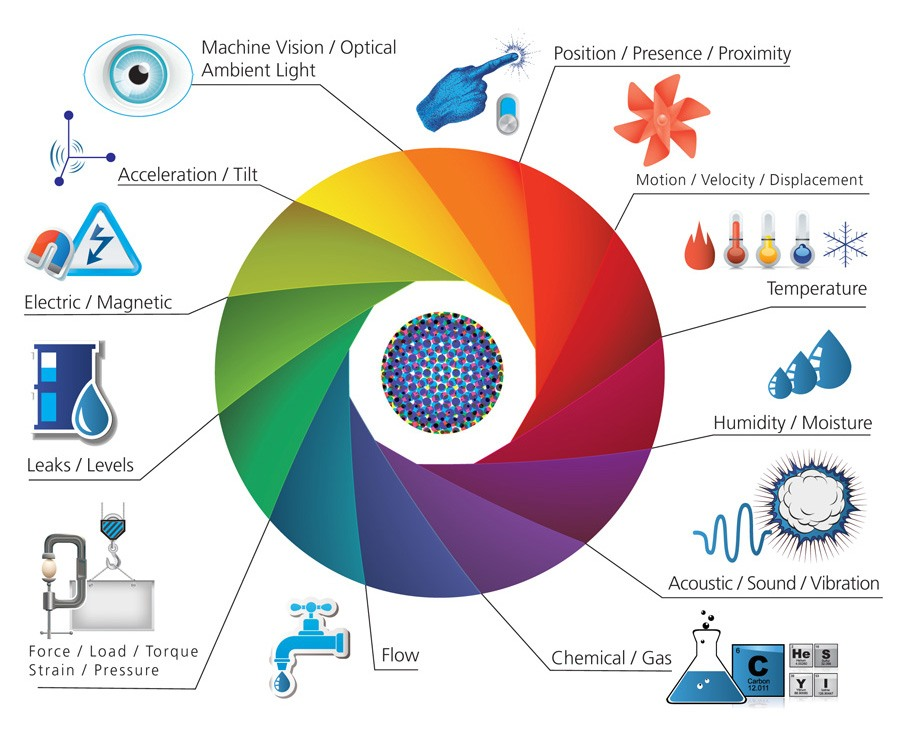
\includegraphics[width=\textwidth]{img/ch-revolution/IOTsensors.jpg}
    \caption[Internet of Things (IoT) sensors \& actuators]{Internet of Things (IoT) sensors \& actuators. We are giving our world a digital nervous system; location data using GPS sensors, eyes and ears using cameras and microphones, along with sensory organs that can measure and record everything (in real-time) from temperature to pressure changes.}
    \source{Harbor Research. \emph{Info-graphic on the \say{Internet of Things}.} \cite{IOT}}
    \label{fig:IOTsensors.jpg}
    \end{figure}
    
    \section{Merging worlds}
    The physical and biological worlds are merging partly thanks to the creation of new materials that are designed to emulate the natural world. The discovery of new classes of recyclable, thermosetting polymers is a significant step towards a more sustainable economy, for example. New materials are now routinely used in medical implants and for tissue engineering. The creation of artificial organs and 3D printing is increasingly being used to create customized structures. The biological and digital worlds overlap most controversially in the world of genetic engineering. Widely-accessible and affordable gene sequencing and editing systems, such as CRISPR/Cas9\footnote{\url{https://ghr.nlm.nih.gov/primer/genomicresearch/genomeediting}}, make it possible to reliably and precisely remove or replace sequences in the genome of plants and animals. The biological and digital worlds are also overlapping in the form of sensors used to monitor personal health and behaviour and to understand and influence brain activity. Advances that might have once been confined to digital systems, like the application of cryptography to blockchain technology to create programmable, secure, and distributed records, are now having widespread impact in the real world. Blockchain, for example, while it may be best known as the framework for virtual currency, can provide new ways to manage land records and track deforestation.

    \section{Shaping the future}

    Neither technology nor the disruption that comes with it is an exogenous force over which humans have no control. All of us are responsible for guiding its evolution, in the decisions we make daily as citizens, consumers, and investors. We should thus grasp the opportunity and power we have to shape the Fourth Industrial Revolution and direct it toward a future that reflects our common objectives and values.\medskip
    
To do this, however, we must develop a comprehensive (and globally shared) view of how technology is affecting our lives. We need to understand how technology is reshaping our economic, social, cultural, and human environments. There has never been a time of more exceptional promise, or one of greater potential peril. Today's decision-makers, however, are too often trapped in traditional, linear thinking, or absorbed by the multiple crises demanding their attention, to think strategically about the forces of disruption and innovation shaping our future.\medskip
    
    In the end, it all comes down to people and values. We need to shape a future that works for all of us by putting people and our environment (nature) first and empowering them. In its most pessimistic, dehumanized form, the Fourth Industrial Revolution may indeed have the potential to "robotize" humanity and thus to deprive us of our heart and soul. However, as a complement to the best parts of human nature - creativity, empathy, stewardship - it can also lift humanity into a new collective and moral consciousness based on a shared sense of destiny. It is incumbent on us all to make sure the latter prevails.
    
    
    \begin{quotation}

      \textit{\say{The only thing that is constant is change.}}
      \begin{flushright}
        \small{--- \textbf{Heraclitus}}
      \end{flushright}
    
    \end{quotation}

